\documentclass{article}

% If you're new to LaTeX, here's some short tutorials:
% https://www.overleaf.com/learn/latex/Learn_LaTeX_in_30_minutes
% https://en.wikibooks.org/wiki/LaTeX/Basics

% Formatting
\usepackage[utf8]{inputenc}
\usepackage[margin=1in]{geometry}
\usepackage[titletoc,title]{appendix}

% Math
% https://www.overleaf.com/learn/latex/Mathematical_expressions
% https://en.wikibooks.org/wiki/LaTeX/Mathematics
\usepackage{amsmath,amsfonts,amssymb,mathtools}

% Images
% https://www.overleaf.com/learn/latex/Inserting_Images
% https://en.wikibooks.org/wiki/LaTeX/Floats,_Figures_and_Captions
\usepackage{graphicx,float}
\usepackage{caption}
\usepackage{subcaption}

% Tables
% https://www.overleaf.com/learn/latex/Tables
% https://en.wikibooks.org/wiki/LaTeX/Tables

% Algorithms
% https://www.overleaf.com/learn/latex/algorithms
% https://en.wikibooks.org/wiki/LaTeX/Algorithms
\usepackage[ruled,vlined]{algorithm2e}
\usepackage{algorithmic}

% Code syntax highlighting
% https://www.overleaf.com/learn/latex/Code_Highlighting_with_minted
\usepackage{minted}
\usemintedstyle{borland}
\usepackage{listings}


% References
% https://www.overleaf.com/learn/latex/Bibliography_management_in_LaTeX
% https://en.wikibooks.org/wiki/LaTeX/Bibliography_Management
\usepackage{biblatex}
\addbibresource{references.bib}

% Title content
\title{AMATH 482 Homework 4}
\author{Rishabh Verma}
\date{March 10th, 2021}

\begin{document}

\maketitle

% Abstract
\begin{abstract}
	Principal component analysis is used to reduce dimension and mine features from the MNIST database of handwritten digits. I then compare how three different classifiers perform when given these labeled features, i.e. linear discriminant analysis (LDA), decision tree classification, and support vector machines. %TODO result
\end{abstract}

% Introduction and Overview
\section{Introduction and Overview}
The MNIST dataset contains labeled scans of handwritten digits. Each scan is a 28x28 pixel image, and each pixel is an 8-bit greyscale value. Each image contains a size-normalized centered digit. There are 60,000 scans in the training set and 10,000 scans in the testing set.

The first goal of this paper is to mine the training set for features which vary across the dataset and correspond with the digits. The second goal is to use these features to perform supervised digit classification. 

%  Theoretical Background
\section{Theoretical Background}
\subsection{Dimensionality reduction and PCA}
PCA is a powerful tool for dimensionality reduction. Consider a series of $n$ observations represented as column vectors $\vec{x_i}$ with $m$ rows. The $m \times n$ matrix $X = \begin{bmatrix}
	\vec{x_1} & \vec{x_2} & ... & \vec{x_n}
\end{bmatrix}$ can be formed. 

Let the mean column be $\vec{x}_\mu$. By computing $X' = X - \vec{x}_\mu \vec{1}^\top$, each column is subtracted from the mean. The resulting matrix has total mean zero, and so we can begin working with variance. Consider the singular value decomposition $X' = U \Sigma V^\top$. The left singular matrix, $U$, is $m \times m$, and contains a basis for the data-space. These basis vectors are the principal components, and are arranged in descending order of variance. The most significant basis vectors are the left-most columns of $U$, and the data can be projected into the $U$-basis via left-multiplication by $U^\top$. Note that this is equivalent to $\Sigma V^\top$. I conclude that the matrix $U^\top=\Sigma V^\top$ will contain in the $ij$-th entry the projection coefficient of the $i$-th data point along the $j$-th principal component.

The process of dimensionality reduction follows from picking a number of dimensions and selecting the corresponding number of singular vectors from the left-most columns of $U$. How do you choose right number of dimensions? One approach comes from the fact that each singular value is directly proportional to the variance along the corresponding singular vector, and so if the singular values drop suddenly in magnitude, the following dimensions do not characterize much of the variance and can be discarded. Another approach is visual; only use enough dimensions that the human eye is able to discern between digits. This latter approach is the one I take. From Figure~\ref{fig:approximations}, it is apparent that no more than 50 dimensions should be necessary to reproduce the structure of the digit. Adding additional dimensions beyond this only seems to sharpen the image, which our classifiers shouldn't rely on.

The first two images in Figure~\ref{fig:approximations} are linear combinations of the mean image and the eigendigits displayed in Figure~\ref{fig:eigendigits}.
\begin{figure}
	\centering
	\begin{subfigure}{.5\textwidth}
		\centering
		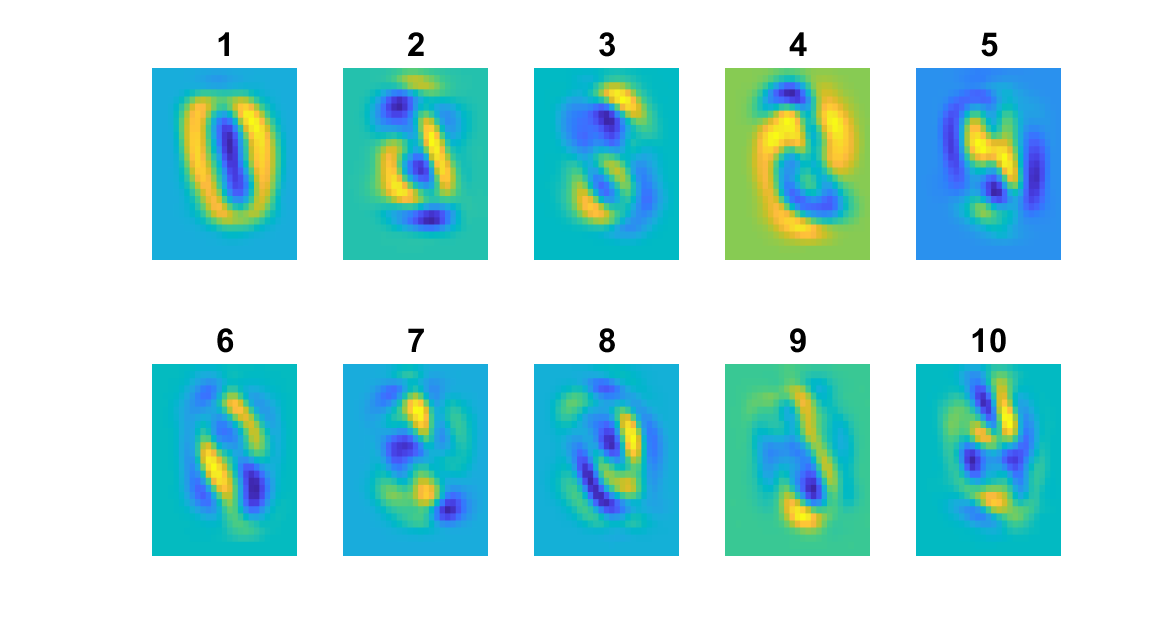
\includegraphics[scale=0.45]{eigendigits}
		\caption{The first 10 eigendigits}    	
		\label{fig:eigendigits}
	\end{subfigure}%
	\begin{subfigure}{.5\textwidth}
		\centering
		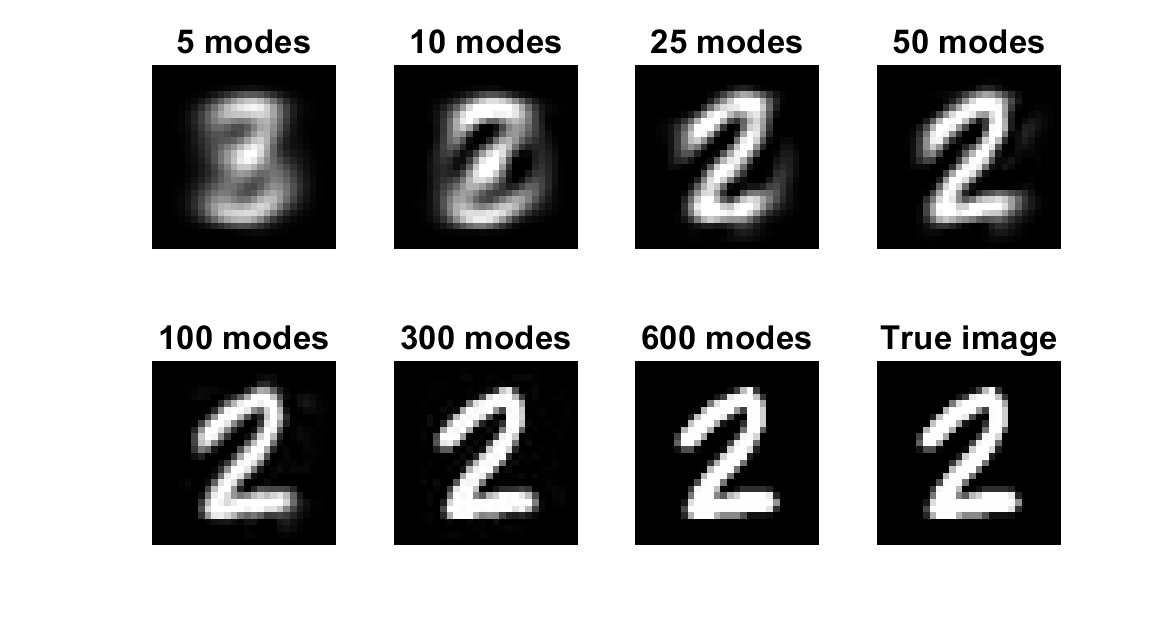
\includegraphics[scale=0.45]{approximations}
		\caption{Eigendigit reconstructions}
		\label{fig:approximations}
	\end{subfigure}
	\caption{Some of the eigendigits, and the approximations they form. }
	\label{fig:fig1}
\end{figure}
\begin{figure}
	\centering
	\;\\
	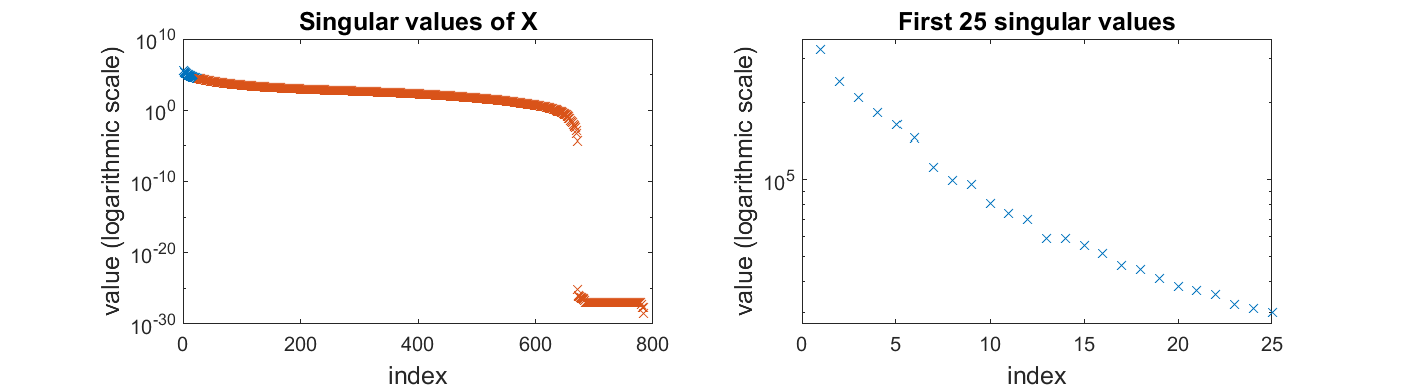
\includegraphics[scale=0.72]{singular_values}
	\caption{Singular values of $X$ (after centering)}
	\label{fig:singular_values}
\end{figure}

\begin{figure}
	\centering
	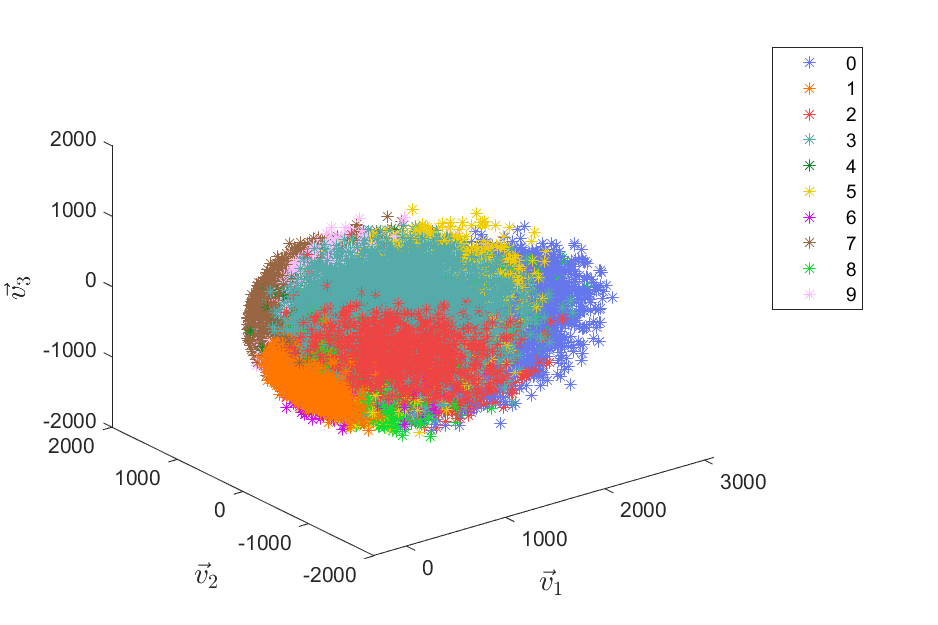
\includegraphics[scale=0.9]{10projections}
	\caption{Projection coefficients along the first three singular vectors, colored by digit}
	\label{fig:10projections}
\end{figure}



% Algorithm Implementation and Development
\section{Algorithm Implementation and Development}


\subsection{Linear classification}
Once the data has been plotted into PCA-space, we can begin the process of classification. In linear classification, we seek to find a vector $\vec{w}$ such that when we project our data onto the line $\text{span}\{\vec{w}\}$, the resulting projection coefficients form clusters corresponding to the labels. We can then threshold an image's projection coefficient to classify it. This is called Linear Discriminant Analysis.

\subsubsection{Finding the right projection image}

Suppose we have $N$ labeled groups of data, where the $j$-th group has mean $\mu_j$. Let $\mu$ be the arithmetic mean of all groups. Define $S_B = \sum_{j=1}^N (\mu_j - \mu)(\mu_j - \mu)^\top$ to measure the covariance between groups, and define $S_W = \sum_{j=1}^N \sum_{\vec{x}_i}(\vec{x}_i-\mu_j)(\vec{x}_i-\mu_j)^\top$ to measure the covariance between means.

The scalar $\vec{w}^\top A w$ characterizes the inner product of the vector $\vec{w}$ before and after transformation with $A$. Consider the quantity $\dfrac{\vec{w}^\top S_B \vec{w}}{\vec{w} S_W \vec{w}}$. Intuitively, this quantity will be maximized when $\vec{w}$ is close to an eigenvector of $S_B$ (the between-class matrix) and far from the eigenvectors of $S_W$ (the within-class matrix). When both of these things are true, I can expect lots of variance between classes and little variance within classes after projecting onto $\vec{w}$. This same vector is the eigenvector corresponding to the largest eigenvalue of the generalized eigenvalue problem in Equation~\ref{eqn:w}.

\begin{equation}
	S_B \vec{w} = \lambda S_W \vec{w}
	\label{eqn:w}
\end{equation}

\subsubsection{Thresholding}

Let $P_i$ be a sorted list containing the projection coefficients of group $i$ onto $\text{span}{\vec{w}}$. Without loss of generality, suppose that if $i < j$, then the projections $P_i$ should be less than the projections $P_j$.

\begin{algorithm}[!h]
	\KwIn{$P_1, P_2$}
	\begin{algorithmic}
		\STATE{set $t_1=\text{length}(P_1), t_2=0$}
		\WHILE{$P_1(t_1) > P_2(t_2)$}
		\STATE{decrement $t_1$}
		\STATE{increment $t_2$}
		\ENDWHILE{}
		\RETURN{the arithmetic mean of $\{t_1,t_2\}$}
	\end{algorithmic}
	\caption{Thresholding 2 groups after LDA}
	\label{alg:lda2}
\end{algorithm}

\begin{algorithm}[!h]
	\KwIn{$P_1, P_2, P_3$}
	\begin{algorithmic}
		\STATE{Set $t_1=\text{length}(P_1), t_2=0$}
		\STATE{Set $t_3=\text{length}(P_2), t_4=0$}
		\WHILE{$P_1(t_1) > P_2(t_2)$}
		\STATE{Decrement $t_1$ by $-2$}
		\STATE{Increment $t_2$}
		\ENDWHILE{}
		\WHILE{$P_2(t_3) > P_3(t_4)$}
		\STATE{Decrement $t_3$}
		\STATE{Increment $t_4$ by $2$}
		\ENDWHILE{}
		\RETURN{the arithmetic means of $\{t_1,t_2\}$ and of $\{t_3,t_4\}$}
	\end{algorithmic}
	\caption{Thresholding 3 groups after LDA}
	\label{alg:lda3}
\end{algorithm}

Algorithm~\ref{alg:lda2} sets the threshold $t$ so that within the training data, the cardinality of $P_1 > t$ approximately matches the cardinality of $P_2 < t$.

Algorithm~\ref{alg:lda3} applies a similar approach to the case where three clusters are projected onto the same line, with slight modification. If Algorithm~\ref{alg:lda2} were applied to $P_1,P_2$ and to $P_2,P_3$, then $P_2$ would be unfairly squished by thresholds on both sides. To counteract this, the algorithm is twice as lenient to $P_2$.



% Computational Results
\section{Computational Results}



LDA performed very well for the digit combinations of $\{0,1\}$ and $\{0,4\}$, with error close to $0.2\%$. LDA performed very poorly for the digit combinations of $\{7,9\}$ and $\{4,9\}$, with error close to $6\%$. Combinations $\{0,1\}$ and $\{7,9\}$ are plotted in Figure~\ref{fig:bestworst}

LDA overall had a tougher time separating three digits at a time. The combination $\{0,1,7\}$ performed the best with less than $9\%$ error, and the combination $\{2,3,6\}$ performed the worst with $65\%$, which is about as bad as randomly guessing. These combinations are plotted in Figure~\ref{fig:triple}.


\begin{figure}[!h]
	\centering
	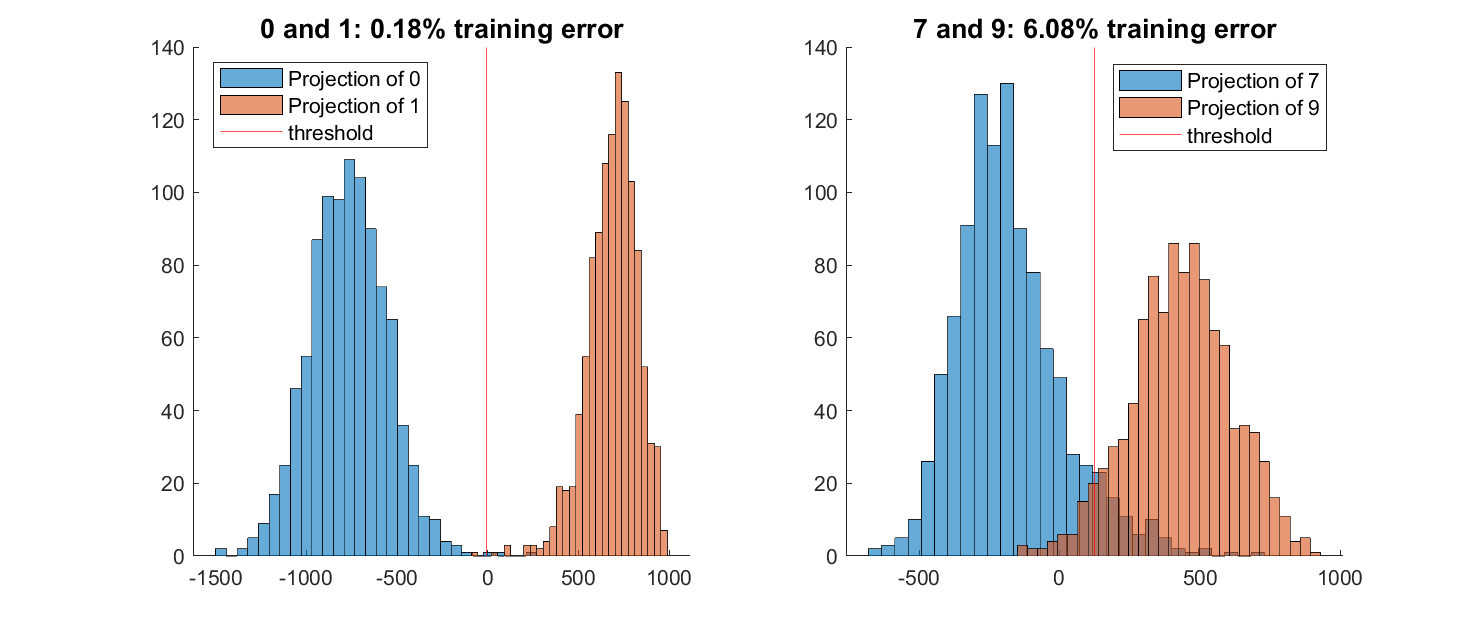
\includegraphics[scale=0.6]{bestworst}
	\caption{The best and worst 2-digit combinations for LDA}
	\label{fig:bestworst}
\end{figure}

\begin{figure}[!h]
	\centering
	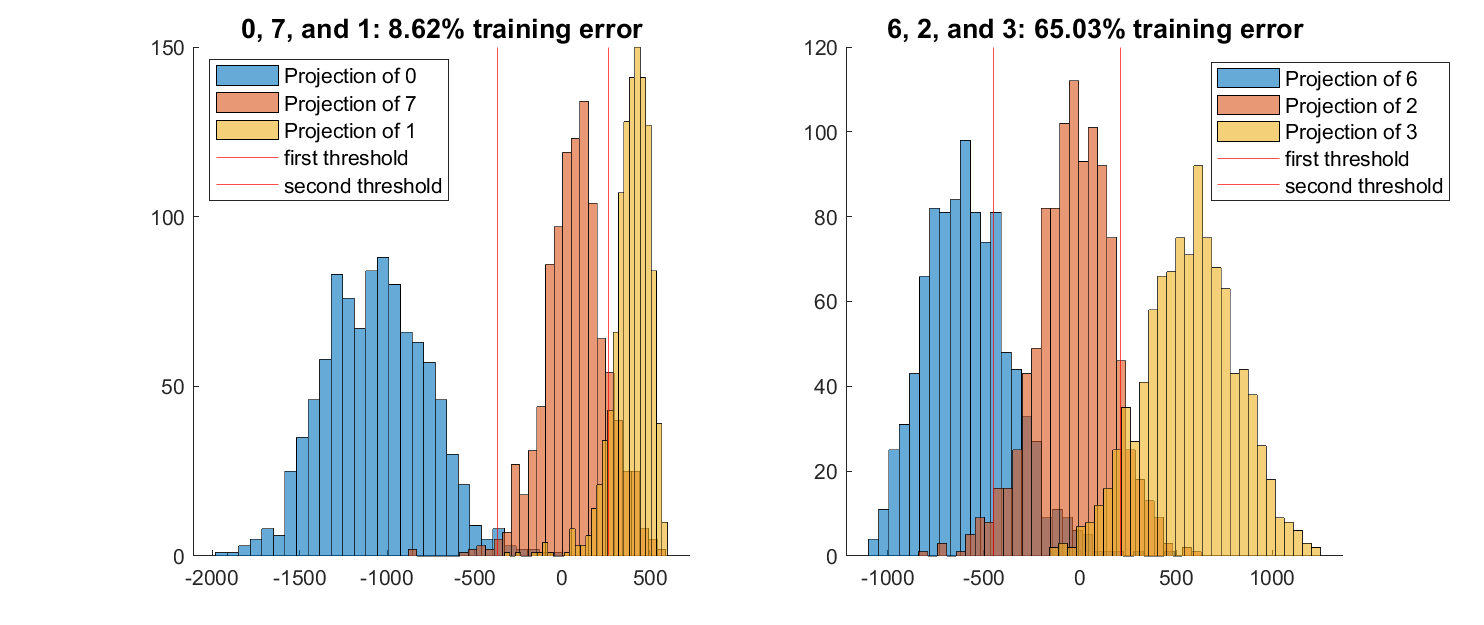
\includegraphics[scale=0.6]{bestworst3}
	\caption{The best and worst 3-digit combinations for LDA}
	\label{fig:triple}
\end{figure}

% Summary and Conclusions

\section{Summary and Conclusions}

Principal Component Analysis performs exceedingly well to mine features in linearizable data. The clusters in Figure~\ref{fig:10projections} show that many defining attributes of digits can be well-characterized by only three singular vectors. This analysis was conducted with a projection onto the first twenty singular vectors, which from Figure~\ref{fig:approximations} does not seem like it would be optimal, and yet it performs quite well.

Linear Discriminant Analysis performs very well to separate easily linearizable data. This includes data with two clusters. Linear Discriminant Analysis also seems to be somewhat effective with data that forms three clusters, though some triples of digits may prove a challenge.



% References
\printbibliography

% Appendices
\begin{appendices}

% MATLAB Functions
\section{MATLAB Functions}

\begin{itemize}
    \item \texttt{[performance, w, threshold] = lda2(a, b, img\_train, label\_train, img\_test, label\_test)} inputs two digits $a,b$ and the associated image/label data sets. The image data should already be projected into PCA-space. The method builds an LDA model by computing the projection vector $\vec{w}$ and the threshold. Output variable \texttt{performance} stores the percentage of errors when testing.
    
    \item \texttt{[performance, w, threshold] = lda3(a, b, c, img\_train, label\_train, img\_test, label\_test)} is similar, except it inputs three digits $a,b,c$ and builds a 3-class LDA model and returns two thresholds.
    
    \item \texttt{[U,S,V] = svd(X)} computes the singular value decomposition of $X$.
\end{itemize}

% MATLAB Codes
\section{MATLAB Code}

\subsection{main.m}
\inputminted{matlab}{main.m}

\subsection{lda2.m}
\inputminted{matlab}{lda2.m}


\subsection{lda3.m}
\inputminted{matlab}{lda3.m}
\end{appendices}
\end{document}